\documentclass{article}
\usepackage{spconf,amsmath,amssymb,graphicx}
\usepackage{booktabs}
\usepackage{cite}
\usepackage{url}
\usepackage{xcolor}
\graphicspath{{figures/}{./}}

% Values still to be filled in by the authors are marked in red; remove before submission.
\newcommand{\tbd}[1]{\textcolor{red}{#1}}

\title{Anchored Flow Matching for EEG Electrode Recovery:\\
Classical Sources, Participant Weighting, and Strong Baselines}
\name{Author Name(s)}
\address{Indian Institute of Technology Mandi\\
Mandi, Himachal Pradesh, India\\
email@example.com}

\begin{document}
\maketitle

\begin{abstract}
Failed EEG electrodes are routinely reconstructed with spherical-spline
interpolation, and deep generative models have recently been proposed as
an alternative. We evaluate graph-informed flow matching (GiFlow) for the
recovery of 50\% of the electrodes in participants unseen during training.
With its published hyperparameters, our implementation is substantially
less accurate than the spline on SEED-IV (normalized mean-squared error,
NMSE, 0.335 vs 0.150). We attribute this to the training mask, the
heat-kernel source of the flow and rapid overfitting, and address each.
The resulting model, which initializes the flow from a per-electrode
mixture of classical estimates, reduces NMSE by 59\% to 0.136 and
outperforms the spline on every seed. Two controls qualify this gain: the
same network trained without flow matching performs equally well (0.133),
and covariance kriging, a linear predictor that requires no training,
performs better (0.116 when training participants are weighted by their
similarity to the test participant). DEAP shows the same pattern, with
kriging reducing NMSE from 0.98 to 0.53 and no learned model surpassing
it. We conclude that learned EEG reconstruction methods should be
benchmarked against such linear baselines, not only against the spline.
\end{abstract}

\begin{keywords}
Electroencephalography, missing channels, flow matching, spherical spline,
kriging
\end{keywords}

\section{Introduction}
\label{sec:intro}

Electrode failure is common in EEG recordings: electrodes detach, the
conductive gel dries, or the contact impedance drifts until the signal is
unusable. Discarding the affected channels is rarely acceptable, because
average referencing, source localization, connectivity analysis and
trained classifiers all assume a fixed montage. Standard preprocessing
pipelines therefore detect bad channels and interpolate them before
analysis \cite{bigdely2015prep}. With dry-electrode and low-cost headsets,
a substantial fraction of the montage may be unreliable at once.

Spherical-spline interpolation \cite{perrin1989spherical} is the standard
method. It fits a smooth surface to the observed potentials on a
spherical head model and evaluates it at the missing sites. It requires no
training data, but it uses only electrode positions and ignores both the
participant-specific covariance between electrodes and the temporal
structure of the signal. Learned models aim to exploit this information.
Convolutional networks have been trained to restore or upsample EEG
channels \cite{svantesson2021virtual}, diffusion models have been applied
to EEG spatial super-resolution \cite{liu2026srgdiff}, and graph-informed
flow matching (GiFlow) \cite{zhang2026giflow} was recently proposed for
spatiotemporal imputation on sensor graphs. GiFlow is well suited to this
task because its flow \cite{lipman2023flow} starts from a graph-diffused
estimate of the missing values rather than from noise, so the network only
needs to learn a correction. However, such methods are usually compared
with the spline alone, and under differing error definitions, montages and
data splits, which makes the actual gain difficult to assess.

We apply GiFlow to recordings in which half of the electrodes have
failed, on SEED-IV \cite{zheng2019emotionmeter} and DEAP
\cite{koelstra2012deap}, with all evaluation on held-out participants. With
the published hyperparameters, its error is more than twice that of the
spline. We analyze the causes and make the following contributions:
\begin{itemize}
\setlength{\itemsep}{0pt}
\item a diagnosis of why GiFlow underperforms on EEG and three remedies
(full-montage training, an anchored source and step-level early stopping)
that together reduce NMSE by 59\% on SEED-IV;
\item a regression control showing that the improvement is due to the
learned correction and the source rather than to flow matching itself;
\item a participant-weighted covariance kriging baseline that outperforms
all learned models we evaluated, on both a 62- and a 32-electrode montage.
\end{itemize}

\section{Method}
\label{sec:method}

\begin{figure*}[t]
\centering
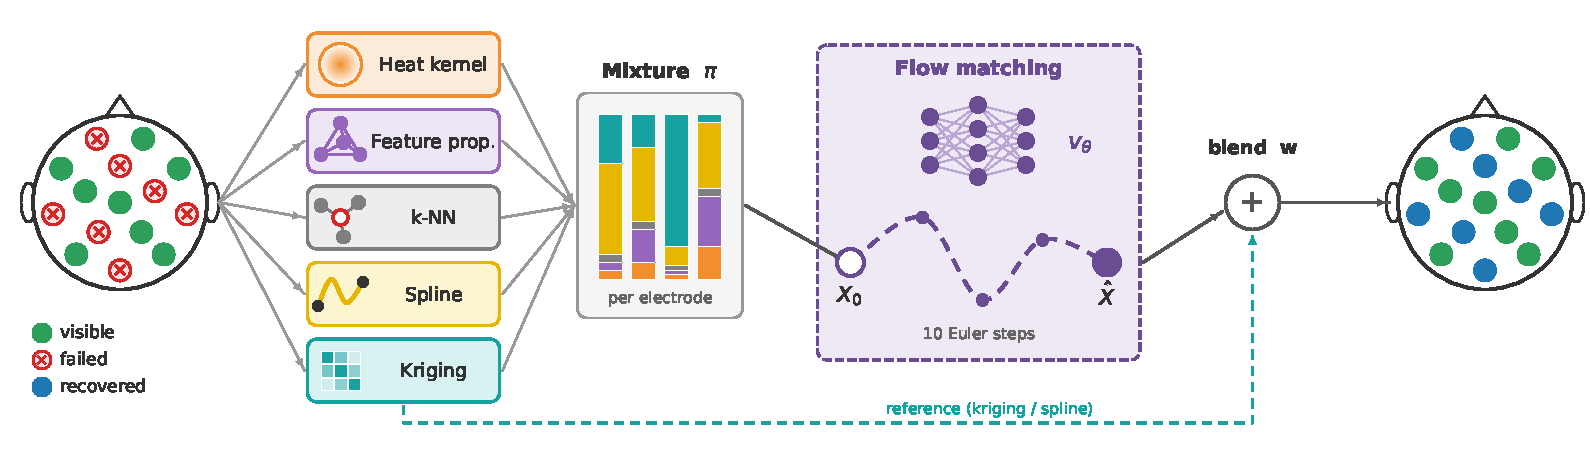
\includegraphics[width=0.9\textwidth]{anchored_flow_pipeline}
\caption{Anchored Flow. Half of the electrodes have failed (red). Five
classical estimators reconstruct them, a per-electrode mixture $\pi$
combines the estimates into the source $X_0$, flow matching transports
$X_0$ to $\hat X$ in 10 Euler steps, and the output is blended with the
kriging or spline estimate using a weight $w$ fitted on validation
participants.}
\label{fig:pipeline}
\end{figure*}

\subsection{Problem setting}

A window $X\in\mathbb{R}^{N\times R}$ contains $N$ electrodes ($N=62$ for
SEED-IV, 32 for DEAP) and $R$ time samples. For each test participant, a
fixed random half of the electrodes is hidden, simulating electrodes that
failed for the entire session; a different half is drawn for each seed.
The model receives $X_{\mathrm{cond}}=M\odot X$, where the binary mask $M$
removes the hidden electrodes, and is evaluated only on the hidden
entries. Training participants have complete montages, reflecting a
laboratory that collects full-montage data once and later repairs
recordings from new participants.

\subsection{GiFlow}

GiFlow \cite{zhang2026giflow} first diffuses the observed values over a
spatial graph (Laplacian $L_s$, derived from electrode correlations in the
training data) and a temporal chain graph ($L_t$),
$X_0=\exp(-\tau_sL_s)\,X_{\mathrm{cond}}\,\exp(-\tau_tL_t)$, with
diffusion times $\tau_s,\tau_t$ fitted in advance. A network $v_\theta$
that alternates spatial and temporal attention with graph message passing
is then trained by flow matching \cite{lipman2023flow} along the linear
path $X_t=(1-t)X_0+tX$, regressing the velocity $X-X_0$ on the hidden
entries. At inference, $v_\theta$ is integrated from $X_0$ in 10 Euler
steps and the observed entries are restored. Since the analysis in
\cite{zhang2026giflow} bounds the imputation error by the transport cost
$\mathbb{E}\|X-X_0\|^2$, a more accurate source is expected to improve the
result.

\subsection{Anchored Flow}

The proposed pipeline is shown in Fig.~\ref{fig:pipeline}. It modifies
GiFlow in three ways.

\emph{Full-montage training.} In our initial protocol, the evaluation mask
was applied to entire recordings, so the evaluated electrodes were also
hidden in all training windows and never served as targets. We instead
keep all electrodes visible in training windows and hide randomly selected
whole electrodes (each with probability 0.5) as targets. Validation and
test windows retain the evaluation mask.

\emph{Anchored source.} The heat-kernel source is replaced by a
per-electrode mixture
\begin{equation}
X_0^{(n)}=\textstyle\sum_k \pi_{nk}\,\hat X_k^{(n)},\qquad
\pi_{n\cdot}=\operatorname{softmax}(\ell_{n\cdot}),
\end{equation}
of $K$ classical estimates $\hat X_k$: the heat kernel, feature
propagation (FP) \cite{rossi2022unreasonable}, $k$-nearest-neighbour
averaging, the spherical spline \cite{perrin1989spherical} computed from
10-05 electrode positions, and covariance kriging. The logits $\ell$ are
fitted on training windows by minimizing the transport cost on hidden
entries and then frozen, allowing each electrode to rely on the estimator
that suits it best. Kriging is the best linear predictor of the hidden
electrodes $h$ given the visible electrodes $v$
\cite{cressie1993statistics},
\begin{equation}
\hat X_h=\Sigma_{hv}(\Sigma_{vv}+\lambda I)^{-1}X_v,
\end{equation}
where $\Sigma$ is the second-moment matrix of the training participants
and $\lambda=10^{-2}$. Whereas the spline imposes a smoothness prior,
kriging uses the empirically observed inter-electrode correlations.

\emph{Step-level early stopping.} With validation once per epoch, the best
checkpoint was invariably the first, indicating that the network overfits
the training participants within a single epoch. We therefore validate
every 25--100 steps, reduce the learning rate to $10^{-4}$, and add weight
decay ($5\times10^{-4}$) and dropout (0.3).

Finally, the output may be blended with the spline or kriging estimate as
$w\hat X_{\mathrm{model}}+(1-w)\hat X_{\mathrm{ref}}$, where $w\in[0,1]$
is fitted by least squares on validation participants; $w$ approaches
zero when the model does not generalize to unseen participants.

\subsection{Participant-weighted kriging}

A single pooled covariance neglects inter-individual differences in head
shape, electrode placement and anatomy. For a new participant, we compute
the correlation matrix $C_v$ of the visible electrodes and assign each
training participant $p$ the weight
$\omega_p\propto\exp(-d_p/(T\,\mathrm{sd}(d)))$, where
$d_p=\|C_v-C^{(p)}_v\|_F$ is computed over the same visible electrodes.
Kriging is then performed with $\sum_p\omega_p\Sigma^{(p)}$. Only the
visible electrodes of the new participant are used, but $C_v$ is
estimated from all of their test windows; the method is therefore
transductive and requires some prior recording from the participant. A
variant fits one covariance per frequency band ($<4$, 4--8, 8--13, 13--30
and $\geq$30~Hz) and sums the band-wise estimates. The temperature $T$ is
selected on validation participants, and the weighted covariance can also
replace the pooled covariance in the anchored source.

\section{Experiments}
\label{sec:experiments}

\textbf{Data.} SEED-IV \cite{zheng2019emotionmeter} contains 15
participants recorded with 62 channels. We use a preprocessed version
(4~s segments at 250~Hz, normalized and soft-clipped to $\pm5$), which we
band-pass filter to 0.5--75~Hz and resample to 200~Hz. DEAP
\cite{koelstra2012deap} contains 32 participants with 32 EEG channels.
From the raw BioSemi recordings, we apply an average reference, band-pass
filter to 0.5--75~Hz, resample to 200~Hz and extract 60 evenly spaced 5~s
segments per participant. Since raw amplitudes differ by two orders of
magnitude across DEAP participants, each recording is centred per channel,
scaled by a single factor (preserving its topography) and soft-clipped
with $5\tanh(x/5)$, consistent with the SEED-IV input. Both datasets are
divided into non-overlapping 100-sample windows (at most 15{,}000).
Participants 7, 10 and 15 are held out for testing and 6 and 12 for
validation; the remainder are used for training. Signals are standardized
using training statistics.

\textbf{Metrics.} NMSE is the squared error summed over all hidden entries,
divided by their total energy; Pearson correlation (PCC) is reported in the
text. Results are given as mean $\pm$ population standard deviation over
seeds 0, 1 and 2. The NMSE definition is consequential: averaging per
window and channel instead emphasizes low-power channels and doubles the
spline's NMSE on our data (0.14 to 0.29). Values obtained under other
definitions or montages are therefore not directly comparable.

\textbf{Implementation.} Hidden size 64, four propagation layers, batch
size 32, Adam with EMA weights; Kaggle T4 GPUs for SEED-IV and an RTX
4050 for DEAP. All quantities other than network weights (mixture logits,
blend weight and kriging temperature) are fitted on training or
validation data only.

\section{Results}
\label{sec:results}

\begin{table}[t]
\centering
\small
\caption{NMSE (lower is better) for 50\% electrode loss on held-out
participants, mean $\pm$ SD over 3 seeds. Learned models are blended with
their reference estimate. --: not evaluated.}
\label{tab:main}
\setlength{\tabcolsep}{3pt}
\begin{tabular}{@{}lcc@{}}
\toprule
Method & SEED-IV & DEAP\\
\midrule
\multicolumn{3}{@{}l}{\emph{Interpolation (no training)}}\\
$k$-NN & 0.291 $\pm$ 0.007 & 0.946 $\pm$ 0.084\\
Feature propagation & 0.322 $\pm$ 0.008 & 0.829 $\pm$ 0.081\\
Spherical spline & 0.150 $\pm$ 0.006 & 0.981 $\pm$ 0.156\\
Kriging, pooled & 0.127 $\pm$ 0.010 & 0.548 $\pm$ 0.060\\
Kriging, participant-weighted & 0.116 $\pm$ 0.009 & 0.532 $\pm$ 0.056\\
\quad per frequency band & \textbf{0.114} $\pm$ 0.008 & --\\
\midrule
\multicolumn{3}{@{}l}{\emph{Learned}}\\
GiFlow, published hyperparam. & 0.335 $\pm$ 0.018 & 1.660 $\pm$ 0.975\\
Anchored Flow, spline source & 0.136 $\pm$ 0.007 & 0.677 $\pm$ 0.058\\
Regression control (no flow) & 0.133 $\pm$ 0.008 & 0.623 $\pm$ 0.032\\
Anchored Flow, + kriging & 0.127 $\pm$ 0.010 & 0.543 $\pm$ 0.053\\
\quad participant-weighted & 0.116 $\pm$ 0.009 & \textbf{0.527} $\pm$ 0.050\\
SRG-style flow, + kriging & 0.127 $\pm$ 0.010 & --\\
\bottomrule
\end{tabular}
\end{table}

\begin{table}[t]
\centering
\small
\caption{Ablation on SEED-IV, adding one modification at a time to GiFlow
with published hyperparameters (NMSE of the model alone and blended).}
\label{tab:ablation}
\setlength{\tabcolsep}{4pt}
\begin{tabular}{@{}lcc@{}}
\toprule
Configuration & Model & Blend\\
\midrule
Published hyperparameters & 0.3350 & --\\
+ full montage, mixed source & 0.2381 & 0.2196\\
+ spline in the mixture & 0.1511 & 0.1452\\
+ validate every 100 steps & 0.1507 & 0.1450\\
+ learning rate $10^{-4}$ & 0.1405 & 0.1394\\
+ weight decay, dropout & 0.1367 & 0.1357\\
+ validate every 25 steps & 0.1364 & 0.1346\\
\bottomrule
\end{tabular}
\end{table}

\textbf{Baseline GiFlow.} With its published hyperparameters, our GiFlow
implementation attains an NMSE of 0.335 on SEED-IV (Table~\ref{tab:main}),
more than twice that of the spline (0.150) and higher than that of
$k$-NN. When the source mixture is learned, the heat kernel receives only
7--10\% of the weight.

\textbf{Effect of the modifications.} Table~\ref{tab:ablation} reports the
modifications cumulatively. Full-montage training with a mixed source
reduces NMSE by 29\%, and including the spline in the mixture, where it
receives 54--56\% of the weight, yields a further 37\% reduction.
Step-level validation alone has no effect, but combined with a lower
learning rate and regularization it moves the best checkpoint to 25--125
steps, and the model alone then outperforms the spline on all three seeds
(0.1335, 0.1463 and 0.1303 vs 0.1482, 0.1576 and 0.1430).

\textbf{Contribution of flow matching.} We trained the same network to
predict $X-X_0$ in a single step at $t=0$, with one-step inference. This
regression control achieves 0.1368 alone and 0.133 blended, matching the
flow. Given a strong source, iterative transport provides no measurable
benefit over a single learned correction.

\textbf{Kriging.} Pooled kriging attains 0.127 without any training, and
participant weighting reduces this to 0.116 (PCC 0.940 vs 0.925 for the
spline), below every learned model. Band-wise covariances give 0.114,
although the variant preferred on validation attains 0.120. On a single
participant with a temporal split, where the covariance transfers
exactly, kriging reaches $0.083\pm0.006$ compared with $0.143\pm0.006$ for
the spline. When kriging is included in the anchored source, it receives
99\% of the mixture weight, and the flow performs no better than kriging
alone (0.127 vs 0.127, and 0.116 vs 0.116 with participant weighting).
The validation-fitted blend weights (0, 0 and 0.30) confirm that the
network learns no correction that generalizes to new participants.
SRGDiff-style residual guidance and step modulation \cite{liu2026srgdiff}
do not change this result.

\textbf{DEAP.} On the sparser 32-electrode montage, the spline performs
close to the trivial zero predictor (0.981, PCC 0.55), whereas kriging
reaches 0.548, and 0.532 with participant weighting (PCC 0.69). GiFlow
with published hyperparameters again underperforms the spline and is
unstable across seeds (0.980, 0.961 and 3.04). The spline-anchored flow
improves on the spline by 31\%, but validation selected the initial or
step-100 weights in all three seeds, so the gain is attributable mainly
to the source mixture (spline 39--43\%, FP 32--33\%, heat kernel
21--24\%). The regression control, which continued to improve for longer,
performs better (0.623). With kriging in the source, the flow remains
within 1\% of kriging alone.

\section{Discussion}
\label{sec:discussion}

Our results lead to three observations. First, protocol choices affected
GiFlow more than any architectural change: a training mask that hid the
evaluated electrodes and per-epoch early stopping each cost more than any
model modification we tested. Second, the source matters more than the
generative model, as the anchored source accounts for most of the
improvement and a network without flow matching performs equally well.
Third, the spherical spline is an insufficient reference: a kriging
predictor based on training covariances, weighted towards participants
similar to the new one, outperformed every learned model on both datasets.
In an earlier pilot (raw data, heat-kernel source, one seed), joint
training on DEAP and SEED-IV improved GiFlow but did not surpass $k$-NN
(macro NMSE 0.613 vs 0.602).

\textbf{Limitations.} The evaluation uses three test participants per
dataset, three seeds, random electrode subsets and short (0.5~s) windows;
differences of about 2\%, such as between the flow and the regression
control, are within seed variation. GiFlow is our reimplementation rather
than the original code, and the cerebellar SEED-IV electrodes CB1/CB2
were placed at I1/I2 for the spline. Contiguous missing regions, very
sparse montages and generative uses such as uncertainty estimation, where
flow models may still be advantageous, were not evaluated, nor were
published diffusion models reproduced under our protocol.

\section{Conclusion}
\label{sec:conclusion}

Anchoring GiFlow to classical estimates, training on the full montage and
applying step-level early stopping reduced its error by 59\% and allowed
it to outperform the spherical spline on unseen participants. However, an
equivalent network without flow matching performs equally well, and
participant-weighted kriging performs better on both SEED-IV and DEAP. We
recommend that studies of learned EEG reconstruction report such linear
baselines under a common error definition.

\section{Compliance with ethical standards}
\label{sec:ethics}

This study used only public datasets \cite{zheng2019emotionmeter,koelstra2012deap};
ethical approval was not required.

\section{Acknowledgments}
\label{sec:acknowledgments}

The authors declare no conflicts of interest. Claude (Anthropic) assisted
with code development and language editing.

\bibliographystyle{IEEEbib}
\bibliography{isbi2027_references}

\end{document}
